\section[弹性力]{\makebox[5em][s]{弹性力}}\label{sec:07.01}

提到弹性力,我们自然会想到弹簧的作用。如图\ref{fig:07.01},它表示
一个弹簧,左端固定在壁上,右端与质量为$ m $的物体连接在一起。
当弹簧处在自然伸长状态时,$ m $并不受力,这个位置称为平衡位
\begin{wrapfigure}[6]{r}{14em}
  \centering
  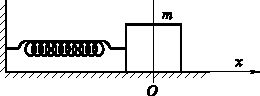
\includegraphics{figure/fig07.01}\\[1em]
  \caption{弹簧的力}
  \label{fig:07.01}
\end{wrapfigure}
置;当把$ m $拉离平衡位置时,$ m $受到弹簧的作用力。这个作用力
的特点是,当把$ m $移到$ O $的右边,即$  x > 0   $的位置时,弹簧力的方
向是向负$ x $的;而当把$ m $移到$ O $的左边,即$ x<0 $的位置时,弹簧力
的方向是向正$ x $的,且力的大小与位移大小成正比。这样,我们可
以把弹簧的作用力写成
\begin{equation}\label{eqn:07.01.01}
  F = - k x
\end{equation}
式中$ x $是$ m $对平衡位置的位移,$ k $叫作弹性系数(或倔强系数),越
大表示弹簧越硬。弹簧的力具有式\eqref{eqn:07.01.01}的性质,这一点也叫胡
克定律。

由式\eqref{eqn:07.01.01}可知弹性力有两个特点:

(1)因为弹性力$ F $的指向总与位移$ x $的方向相反,故弹性力
$ F $总是指向平衡位置,总是力图把质点拉回到平衡位置;
% 199.jpg

(2)因为$ F $的数值大小正比于位移$ x $的大小,所以$ m $偏离平
衡点越远,则它受到的拉回平衡点的力也越大。

因此,可以看到,在弹性力$ F $作用下的质点,其基本的运动
形式是在平衡点附近来回振荡,它是一种被“束缚”在平衡点附
近的运动。

\begin{wrapfigure}[10]{r}{13em}
  \centering
  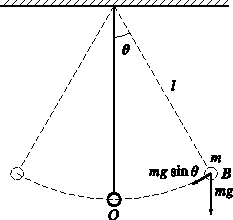
\includegraphics{figure/fig07.02}
  \caption{弹簧}
  \label{fig:07.02}
\end{wrapfigure}
除了弹簧外,其他的力也可能具有\eqref{eqn:07.01.01}的形式。如图
\ref{fig:07.02}\;所示的单摆,如将小球从平衡点$ O $拉到$ B $点再松手,小球将在
平衡位置$ O $点附近往复摆动。它的结构虽与上述振子$ m $完全不
同,但它们的运动性质是十分相似的。我们以角位移$ \theta $作为描写
小球位置的变量,并规定小球在平衡位置右方时,$ \theta $为正;在左
方时,$ \theta $为负。如果偏角$ \theta $很小,小球受到的重力与绳的张力的
合力为
\begin{equation}\label{eqn:07.01.02}
  F = - m g \sin \theta \approx - m g \theta
\end{equation}
式中负号表示$ F $与角位移方向相反。当小球偏向右方,即 $ \theta > 0  $
时,$ F $指向左方$ \left( F < 0 \right) $;当偏向左方,即$  \theta < 0   $时,$ F $指向右方
$ \left( F > 0 \right) $。亦即$ F $永远指向平衡位置,且$ F $大小与角位移的大小
成正比。

可见,单摆所受的虽不是弹性力,但式\eqref{eqn:07.01.02}在形式上与式
\eqref{eqn:07.01.01}完全相似。我们把这种与弹性力具有相似表达式的力,叫
做准弹性力。

这类弹性力的实例,还可以举出许多。例如琴弦的颤动,
树木的摇曳,分子的振动等,都是在准弹性力作用下的运动。一
般质点在其稳定的平衡点附近的运动,大都是准弹性力作用下的
% 200.jpg
运动。现在我们来证明这一点。

\clearpage
上章讨论一维运动的一般性质时已指出,所谓稳定的平衡点,
即势能曲线中的极小点。例如图7.3表示的势能曲线, $ x = x _ { 0 }   $即是
一个稳定的平衡位置。能量为$ E = V _ 0 $的质点可以在$  x = x _ { 0 }   $处于静
止状态。如果给质点添加一点能量,它将在$ x $附近来回振荡作束
缚运动。按一般理论式\eqref{eqn:06.05.01},这个运动所受的力为

\begin{figure}[h]
  \centering
  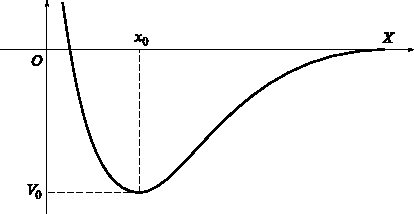
\includegraphics{figure/fig07.03}
  \caption{稳定的平衡状态}
  \label{fig:07.03}
\end{figure}

\begin{equation}\label{eqn:07.01.03}
  F = - \frac { \dif V } { \dif x }
\end{equation}

由于质点只在$ x $附近运动,故可以把势能函数$ V\left(x\right) $在$  x _ { 0 }   $点
附近作泰勒展开
\begin{equation}\label{eqn:07.01.04}
  \begin{aligned}
    V \left( x \right) = V _ { 0 } & + \left ( \frac { \dif V } { \dif x } \right ) _ { x = x _ { 0 } } \left( x - x _ { 0 } \right)                                                 \\
                                   & + \frac { 1 } { 2 } \left( \frac { \dif ^ { 2 } V } { \dif x ^ { 2 } } \right) _ { x = x _ { 0 } } \left( x - x _ { 0 } \right) ^ { 2 } + \dots
  \end{aligned}
\end{equation}
因为$ x $是$ V\left(x\right) $的极小点,故
\begin{equation*}
  \left( \frac { \dif V } { \dif x } \right) _ { x = x _ { 0 } }  = 0
\end{equation*}
所以,对于在$ x _ { 0 } $附近的运动,忽略式\eqref{eqn:07.01.04}中$ \left( x - x _ { 0 } \right) ^ { 3 }  $以后的
项,势能函数可近似为

% 201.jpg
\clearpage
~\vspace{-2.5em}
\begin{equation}\label{eqn:07.01.05}
  V \left( x \right) = V _ { 0 } + \frac { k } { 2 } \left( x - x _ { 0 } \right) ^ { 2 }
\end{equation}
\begin{align}\label{eqn:07.01.06}
  \beforetext{其中} k = \left( \frac { \dif ^ { 2 } V } { \dif x ^ { 2 } } \right) _ { x = x _ { 0 } }
\end{align}
它是个大于零的数。将式\eqref{eqn:07.01.05}代入式\eqref{eqn:07.01.03},就得到
\begin{equation}\label{eqn:07.01.07}
  F = - k \left( x - x _ { 0 } \right)
\end{equation}
可见,只要把平衡位置$ x _ 0 $取为原点,它的形式与式\eqref{eqn:07.01.01}就完全
一样了。这就证明了物体在其平衡位置所受到的力,都具有弹性
力的性质。

弹性力\lhbrak 式\eqref{eqn:07.01.01}\rhbrak 的势能函数是
\begin{equation}\label{eqn:07.01.08}
  V = \frac { 1 } { 2 } k x ^ { 2 }
\end{equation}
\begin{wrapfigure}[8]{r}{12.5em}
  \centering
  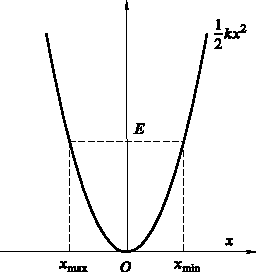
\includegraphics{figure/fig07.04}
  \caption{弹性力的势能函数}
  \label{fig:07.04}
\end{wrapfigure}
实际上,取$  V _ { 0 } = 0   $,$  x _ { 0 } = 0   $代入式
\eqref{eqn:07.01.05},即得到上式。

势能\lhbrak 式\eqref{eqn:07.01.08}\rhbrak 的曲线示
于图\ref{fig:07.04}\;中。由图可见,在一个严格的弹性力作用下的质点只可
能作束缚运动,对任何大的能量$ E $,质点都不能作自由运动,而
只能在下列有限范围内运动,即
{\setlength{\mathindent}{4em}
\begin{equation*}
  x _ { \text { min } } \leqslant x \leqslant x _ { \text { max } }
\end{equation*}
\begin{align*}
      \beforetext{其中} x _ { \text { min } } &= - \sqrt { \frac { 2 E } { k } } \\
  x _ { \text { max } } &= + \sqrt { \frac { 2 E } { k } }
\end{align*}}
\vspace{-2em}
